

%%%%%%%%%%%%%%%%%%%%%%%%%%%%%%%%%%%%%%%%%%%%%%%%%%%%%%%%%%%%%%%%%%%%%%%%%%%%%%%%%%%%%%%%%%%%%%%%%%%%

\begin{figure}[h!]

\begin{center}

    \caption{Volume Under the ``ROC Surface''} \label{fig:volume1}

    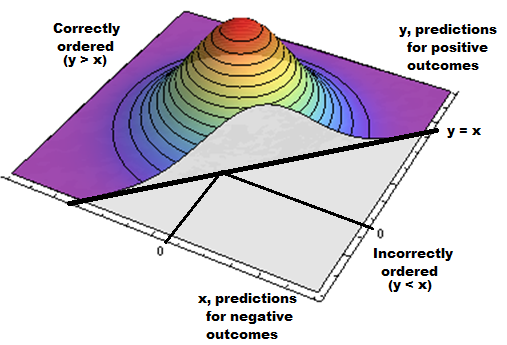
\includegraphics[scale=  0.500000]{Figs/Volume/AUROC_vol_3.png}

\end{center}

\footnotesize

    \textbf{Volume Under the ``ROC Surface'':}
    With the AUROC defined in the form $A = Prob{\left\{ y > x \right\}}$, it is clear that it can be visualized as the volume of the probability mass under the surface of the joint distribution of classification variables from positive and negative outcomes.

\end{figure}



%%%%%%%%%%%%%%%%%%%%%%%%%%%%%%%%%%%%%%%%%%%%%%%%%%%%%%%%%%%%%%%%%%%%%%%%%%%%%%%%%%%%%%%%%%%%%%%%%%%%

